\documentclass[12pt]{article}
\usepackage{graphics}
\newcommand{\kg}{\mathrm{kg}}
\newcommand{\m}{\mathrm{m}}
\newcommand{\s}{\mathrm{s}}
\renewcommand{\deg}{\mathrm{deg}}
\newcommand{\cm}{\mathrm{cm}}
\newcommand{\mps}{\m\,\s^{-1}}
\newcommand{\mpss}{\m\,\s^{-2}}
\newcommand{\kgpmmm}{\kg\,\m^{-3}}
\newcommand{\N}{\mathrm{N}}
\newcommand{\J}{\mathrm{J}}
\newcommand{\Npmm}{\N\,\m^{-2}}
\newcommand{\tv}[1]{\mathbf{\vec{#1}}}
\newcommand{\dd}{\mathrm{d}}
\newcommand{\cell}[1]{\texttt{{#1}}}
\newcounter{problem}
\addtolength{\oddsidemargin}{-1in}
\addtolength{\textheight}{\headheight}
\setlength{\headheight}{0in}
\addtolength{\textheight}{\headsep}
\setlength{\headsep}{0in}
\setlength{\marginparwidth}{2in}
\begin{document}

\section*{NYU Physics 1---midterm exam}

Wednesday 2008 October 15 in lecture.

~ \vfill ~

\section*{Name:}

~ \vfill ~

\begin{equation}
\tv{v} = \frac{\dd}{\dd t}\tv{r}
\quad ; \quad
\tv{a} = \frac{\dd}{\dd t}\tv{v}
\end{equation}
\begin{equation}
a_{\mathrm{circ}} = \frac{v^2}{R} = \omega^2\,R
\end{equation}
\begin{equation}
\tv{F} = m\,\tv{a}
       = \frac{\dd}{\dd t}\tv{p}
       = \frac{\dd}{\dd t}(\gamma\,m\,\tv{v})
\end{equation}
\begin{equation}
|\tv{F}_{\mathrm{grav}}| = \frac{G\,M\,m}{r^2} = m\,g
\end{equation}
\begin{equation}
|\tv{F}_{\mathrm{static}}| \leq \mu\,|\tv{N}|
\quad ; \quad
|\tv{F}_{\mathrm{kinetic}}| = \mu\,|\tv{N}|
\end{equation}
\begin{equation}
\Delta U = m\,g\,\Delta h
\quad ; \quad
K = \frac{1}{2} m\,v^2
\end{equation}

\clearpage

\paragraph{Problem~\theproblem}\refstepcounter{problem}%
This is the layout for a planned roller coaster; one that satisfies
all standard safety concerns.  Draw a free-body diagram for the
roller-coaster cart when it gets to the point marked A.\\
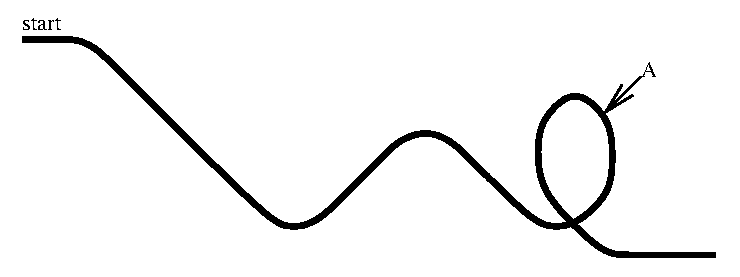
\includegraphics{../eps/roller_coaster.eps}

~ \vfill ~

\paragraph{Problem~\theproblem}\refstepcounter{problem}%
In lecture we considered a car sliding around a banked circular turn
at constant speed, in the absence of friction.  Now imagine that the
car has static friction acting for transverse forces (that is,
opposing sliding up or down the bank) with a coefficient of $0.2$.
Draw the free-body diagram for the car when it is going around the
turn at the maximum speed at which the car can go without sliding
uphill or downhill.

~ \vfill ~

\clearpage

\paragraph{Problem~\theproblem}\refstepcounter{problem}%
Compute the velocity of the Space Shuttle in its orbit around the
Earth in units of $\mps$.  Assume it is orbiting very close to the
surface of the Earth (not a bad approximation, as we discussed in
class).  If you need to assume anything else, state your assumptions
explicitly.

~ \vfill ~

\paragraph{Problem~\theproblem}\refstepcounter{problem}%
The Sun orbits the Milky Way on a close-to-circular orbit at a speed
of $2\times 10^5\,\mps$ and a distance of $R= 3\times 10^{20}\,\m$.
What is the orbital period of the Sun around the Milky Way?

~ \vfill ~

\clearpage

\paragraph{Problem~\theproblem}\refstepcounter{problem}%
Imagine you plan a interstellar voyage in which you increase your
momentum at constant force $F$ (in a constant direction) for a time
$T$, where $T$ is long enough that you have to use the relativistic
formula for momentum.  What speed $v$ do you end up going at the end
of the period, relative to the frame at which you were at rest when
you started?

~ \vfill ~

\paragraph{Problem~\theproblem}\refstepcounter{problem}%
A bullet of mass $m$ moving at speed $v$ hits and lodges in a block of
mass $M$ that is initially at rest.  The combined system ends up
moving at some new speed $v'$.  Ignore all other forces and conserve
linear momentum.  What is the change in kinetic energy (total kinetic
energy after minus total kinetic energy in all components before)?

~ \vfill ~

\clearpage

\paragraph{Problem~\theproblem}\refstepcounter{problem}%
Imagine a particle of mass $m$ moving back and forth in the $x$
direction according to the equation
\begin{equation}
x(t)= A\,\cos\left(\omega\,t\right) \quad .
\end{equation}
What is the force as a function of time $F(t)$?

~ \vfill ~

\paragraph{Problem~\theproblem}\refstepcounter{problem}%
What formulae should go into cells \cell{E9} and \cell{F9} in this
spreadsheet, which is integrating a trajectory?  State your formulae
in terms of the cell numbers (such as ``\cell{I8}''), not variables
(such as ``$a_x$''). \\
\resizebox{\textwidth}{!}{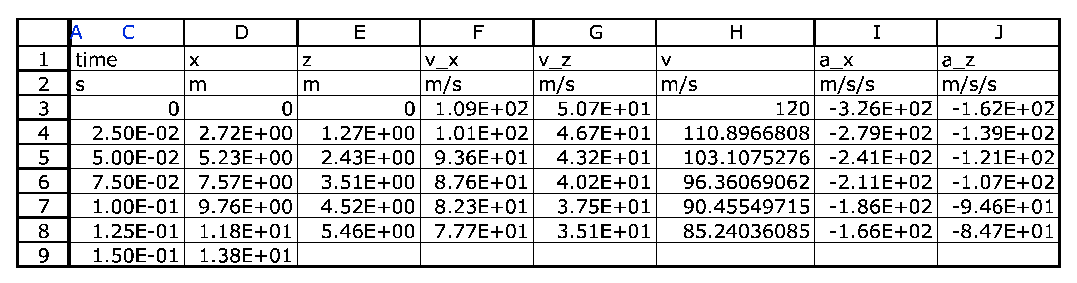
\includegraphics{../xls/exam.eps}}

~ \vfill ~

\clearpage

\paragraph{Problem~\theproblem}\refstepcounter{problem}%
For this block-and-pulley system, I started to give---in lecture---an
argument that the $7\,\kg$ block will accelerate downwards.  Give this
argument, in words.
\marginpar{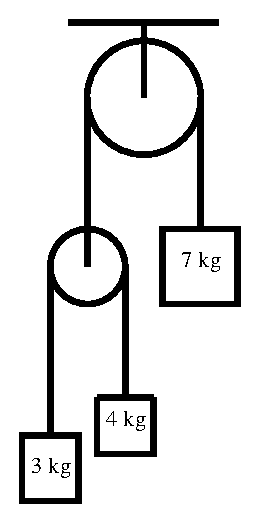
\includegraphics{../eps/blocks_3_4_7.eps}}%

~ \vfill ~

\end{document}
